\chapter{Datasets, Simulated Samples and Triggers}
\label{chap:Samples}

This analysis is based on data collected by the \ac{CMS} experiment in 2016-2018 from pp collisions at a center-of-mass energy of 13 TeV corresponding to an integrated luminosity of 138 fb$^{-1}$. Approximately 30 simultaneous pp collisions were occurring per 25 ns. Based on online selection criteria, fully reconstructed collision data that contain high-level physics objects are divided into ``\acp{PD}''. The \acp{PD} that make use of lepton information for selection include ``DoubleEG'', ``DoubleMu'', ``MuonEG'', ``SingleElectron'', and ``SingleMuon'' for the 2016 and 2017 data-taking era. In 2018, ``SingleElectron'' and ``DoubleEG'' were replaced by ``EGamma''. The names of these \acp{PD} reflect the selection criteria. In addition to these \acp{PD}, \ac{MC} samples are also generated to model both signal and background processes, which are described in \autoref{sec:Signals} and \autoref{sec:Backgrounds}, respectively. To account for the different data-taking conditions across the years, all \ac{MC} samples are generated separately for each year. \ac{HLT} triggers are used to select events offline, which is described in \autoref{sec:Triggers}.
%%%%%%%%%%%%%%%%%%%%%%%%%%%%%%%%%%%%%%%%%%%%%%%%%%%%%%%%%%%
%%%%%%%%%%%%%%%%%%%%%%%%%%%%%%%%%%%%%%%%%%%%%%%%%%%%%%%%%%%

\section{Signal Samples}
\label{sec:Signals}

\begin{table}[t]
\sffamily
\centering
\caption{Summary of relevant dimension-6 operators considered in this analysis. Here, $\varepsilon$ is the two dimensional Levi-Civita symbol, $\gamma^\mu$ the Dirac gamma matrices, and $\sigma^{\mu\nu}=\frac{\textsf{i}}{2}[\gamma^\mu,\gamma^\nu]$. The l and q denote left-handed doublets, whereas u and e denote right-handed singlets. The indices $i$ and $j$ are lepton flavor indices that run from 1 to 2 with $i \neq j$; $m$ and $n$ are quark flavor indices with the condition that one of them is 3 and the other one is 1 or 2.}
\begin{tabular}{cccl}
\toprule
Lorentz Structure & \multicolumn{3}{c}{Operator}\\
\midrule
\multirow{4}{*}{vector} & $\textsf{O}_{\textsf{lq}}^{(1)ijmn}$ &=& $(\overline{\textsf{l}}_i\gamma^\mu\textsf{l}_j)
 (\overline{\textsf{q}}_m\gamma_\mu\textsf{q}_n)$
 \\
 & $\textsf{O}_{\textsf{lu}}^{ijmn}$ &=& $(\overline{\textsf{l}}_i\gamma^\mu\textsf{l}_j)
 (\overline{\textsf{u}}_m\gamma_\mu\textsf{u}_n)$
 \\  
 & $\textsf{O}_{\textsf{eq}}^{ijmn}$ &=& $(\overline{\textsf{e}}_i\gamma^\mu\textsf{e}_j)
 (\overline{\textsf{q}}_m\gamma_\mu\textsf{q}_n)$
 \\ 
 & $\textsf{O}_{\textsf{eu}}^{ijmn}$ &=& $(\overline{\textsf{e}}_i\gamma^\mu\textsf{e}_j)
 (\overline{\textsf{u}}_m\gamma_\mu\textsf{u}_n)$
 \\ \midrule
\multirow{1}{*}{scalar} & $\textsf{O}_{\textsf{lequ}}^{(1)ijmn}$ &=& $(\overline{\textsf{l}}_i\textsf{e}_j)\;\varepsilon\;
 (\overline{\textsf{q}}_m\textsf{u}_n)$
 \\ 
 \multirow{1}{*}{tensor} & $\textsf{O}_{\textsf{lequ}}^{(3)ijmn}$ &=& $(\overline{\textsf{l}}_i \sigma^{\mu\nu}\textsf{e}_j)\;\varepsilon\;
 (\overline{\textsf{q}}_m\sigma_{\mu\nu}\textsf{u}_n)$
 \\ \bottomrule
\end{tabular}
\label{tab:dimension6}
\end{table}

In this analysis, New Physics is described by Dimension-6 \ac{EFT} operators,

\begin{equation}
\label{eq:0}
\mathcal{L}=\mathcal{L}_{\textsf{SM}}^{(4)} + \frac{1}{\Lam^2}\sum_{a}\WC{(6)}{a}\OP{(6)}{a}+O\left( \frac{1}{\Lam^4}\right).
\end{equation}  

Among many of the Dimension-6 operators in Warsaw basis~\cite{Grzadkowski:2010es,Aguilar-Saavedra:2018ksv}, a total of 6 operators are considered, which are summarized in Table~\ref{tab:dimension6}. To reduce the number of free parameters, the permutations of fermion flavors are combined. Taking $\emut{u}$ vertex as an example, the \acp{WC} are parameterized in the following way:

\begin{eqnarray}
\label{eq:1:0}
 \textsf{C}_{\textsf{lq}}
 &=& \textsf{C}_{\textsf{lq}}^{(1)1213}
 + \textsf{C}_{\textsf{lq}}^{(1)2113}
 + \textsf{C}_{\textsf{lq}}^{(1)1231}
 + \textsf{C}_{\textsf{lq}}^{(1)2131}
 ,\\
\label{eq1:1}
 \textsf{C}_{\textsf{lu}}  
 &=& \textsf{C}_{\textsf{lu}}^{1213}
 + \textsf{C}_{\textsf{lu}}^{2113}
 + \textsf{C}_{\textsf{lu}}^{1231}
 + \textsf{C}_{\textsf{lu}}^{2131}
 ,\\
 \label{eq:1:2}
 \textsf{C}_{\textsf{eq}}
 &=& \textsf{C}_{\textsf{eq}}^{1213}
 + \textsf{C}_{\textsf{eq}}^{2113}
 + \textsf{C}_{\textsf{eq}}^{1231}
 + \textsf{C}_{\textsf{eq}}^{2131}
 ,\\
 \label{eq:1:3}
 \textsf{C}_{\textsf{eu}}  
 &=& \textsf{C}_{\textsf{eu}}^{1213}
 + \textsf{C}_{\textsf{eu}}^{2113}
 + \textsf{C}_{\textsf{eu}}^{1231}
 + \textsf{C}_{\textsf{eu}}^{2131},
\end{eqnarray}

\begin{eqnarray}
\label{eq:1:4}
 \textsf{C}_{\textsf{lequ}}^{(1)}  
 &=& \textsf{C}_{\textsf{lequ}}^{(1)1213}
 + \textsf{C}_{\textsf{lequ}}^{(1)2113}
 + \textsf{C}_{\textsf{lequ}}^{(1)1231}
 + \textsf{C}_{\textsf{lequ}}^{(1)2131}
 ,\\
\label{eq:1:5}
 \textsf{C}_{\textsf{lequ}}^{(3)}
 &=& \textsf{C}_{\textsf{lequ}}^{(3)1213}
 + \textsf{C}_{\textsf{lequ}}^{(3)2113}
 + \textsf{C}_{\textsf{lequ}}^{(3)1231}
 + \textsf{C}_{\textsf{lequ}}^{(3)2131}. 
\end{eqnarray}

Additionally, all vector-like operators are combined,

\begin{eqnarray}
\label{eq:1:6}
 \OP{\textsf{vector}}{\emut{u}}&=&\OP{}{\textsf{lq}}+\OP{}{\textsf{lu}}+\OP{}{\textsf{eq}}+\OP{}{\textsf{eu}},\\
\label{eq:1:7}
 \OP{\textsf{scalar}}{\emut{u}}&=&\OP{(1)}{\textsf{lequ}}+\textsf{h.c},\\
\label{eq:1:8}
 \OP{\textsf{tensor}}{\emut{u}}&=&\OP{(3)}{\textsf{lequ}}+\textsf{h.c},
\end{eqnarray}

which results in 6 independent \acp{WC}: $\WC{\textsf{vector}}{\emut{u}},~\WC{\textsf{scalar}}{\emut{u}},~\WC{\textsf{tensor}}{\emut{u}},~\WC{\textsf{vector}}{\emut{c}},~\WC{\textsf{scalar}}{\emut{c}},~\WC{\textsf{tensor}}{\emut{c}}.$  

To generate signal \ac{MC} samples, the effective Lagrangian described above is implemented using the SmeftFR v2~\cite{Dedes:2019uzs} model, and saved in the ``UFO'' format~\cite{Degrande:2011ua}. Additionally, all the \acp{WC} are set to 1 with $\Lam$ = 1 TeV in the UFO, which then interfaces with the \textsc{FeynRules}~\cite{Christensen:2008py} package to calculate Feynman diagrams. The output of the \FR~is used in \ac{ME} event generator \MG~v2.4.2~\cite{Alwall:2014hca} to generate events at \ac{LO}. 

\begin{figure}[tbh!]
 \begin{center}
 \begin{tabular}{cc}
 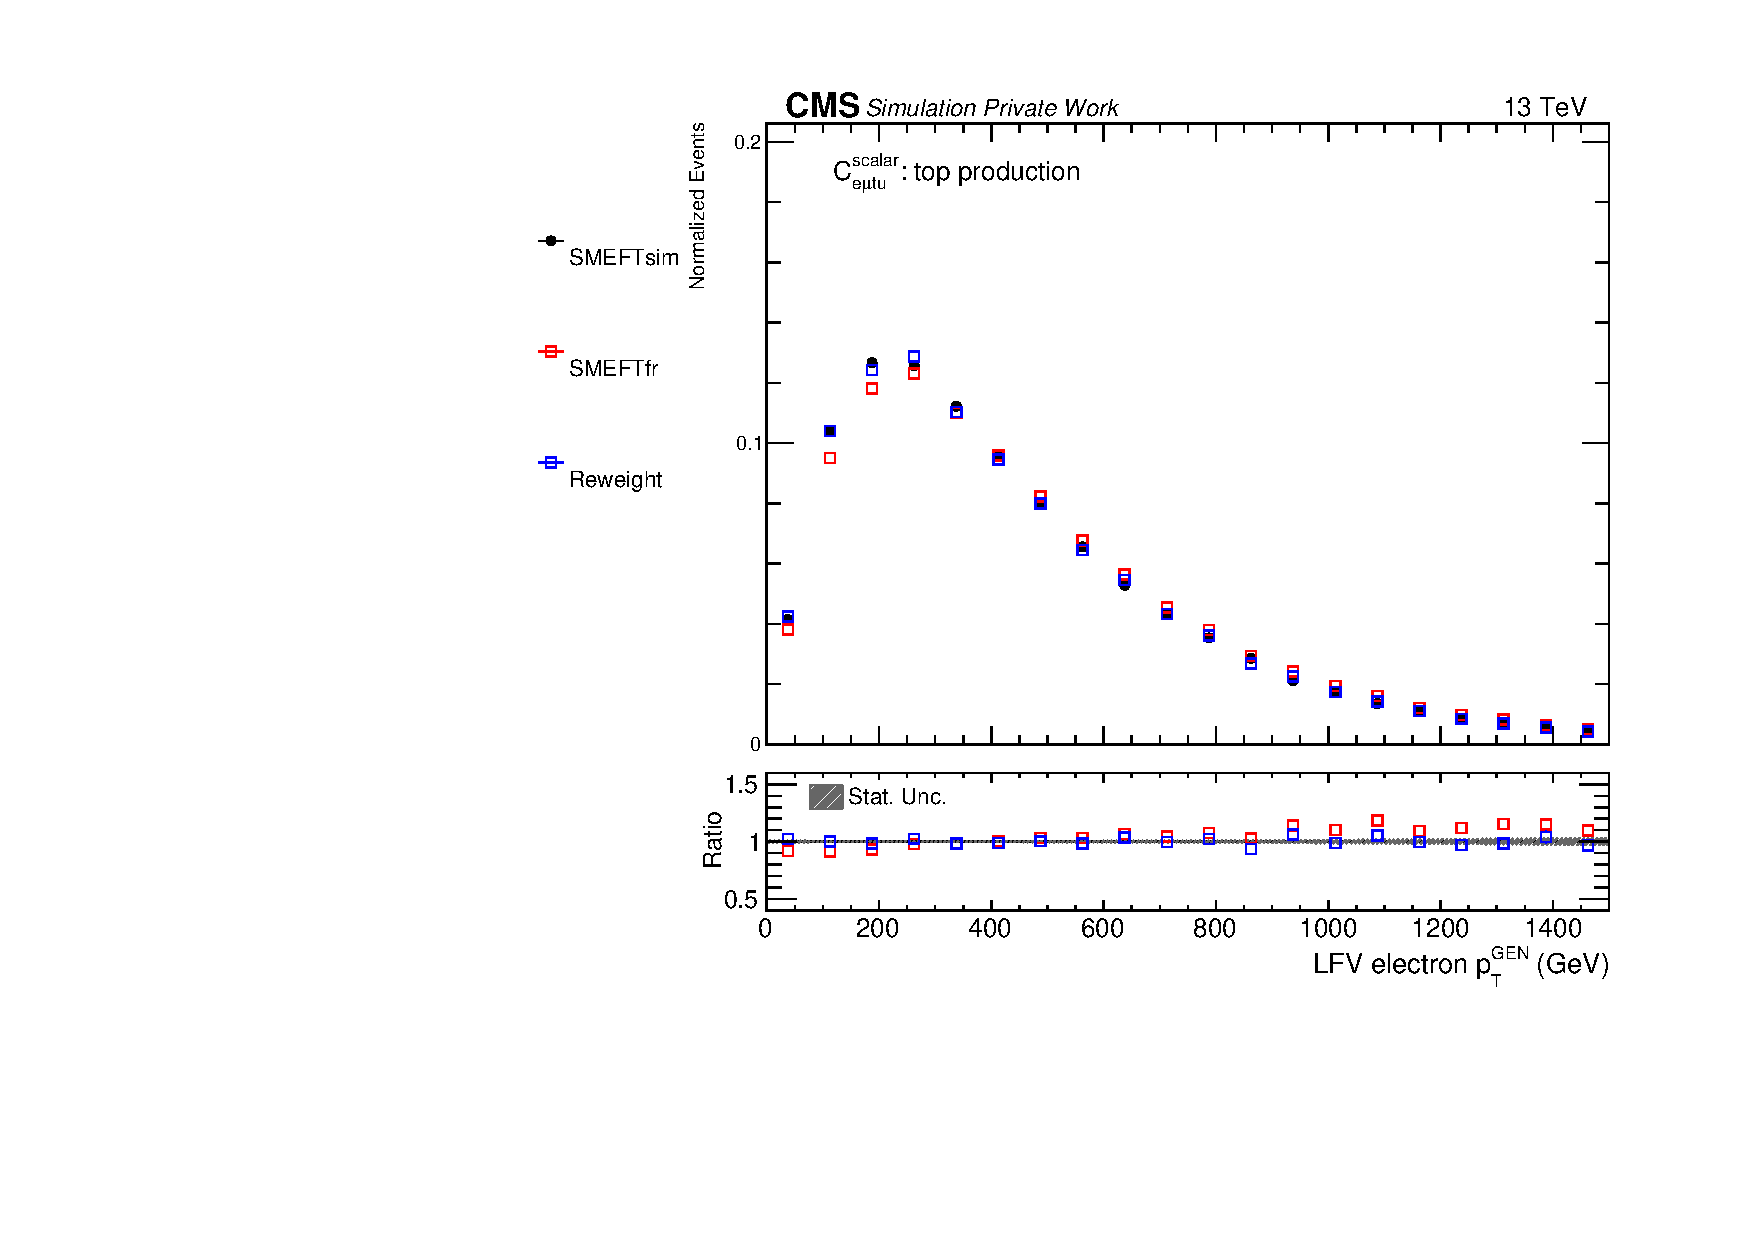
\includegraphics[width=0.48\textwidth]{figures/Part3/Samples/LFVePt}&
 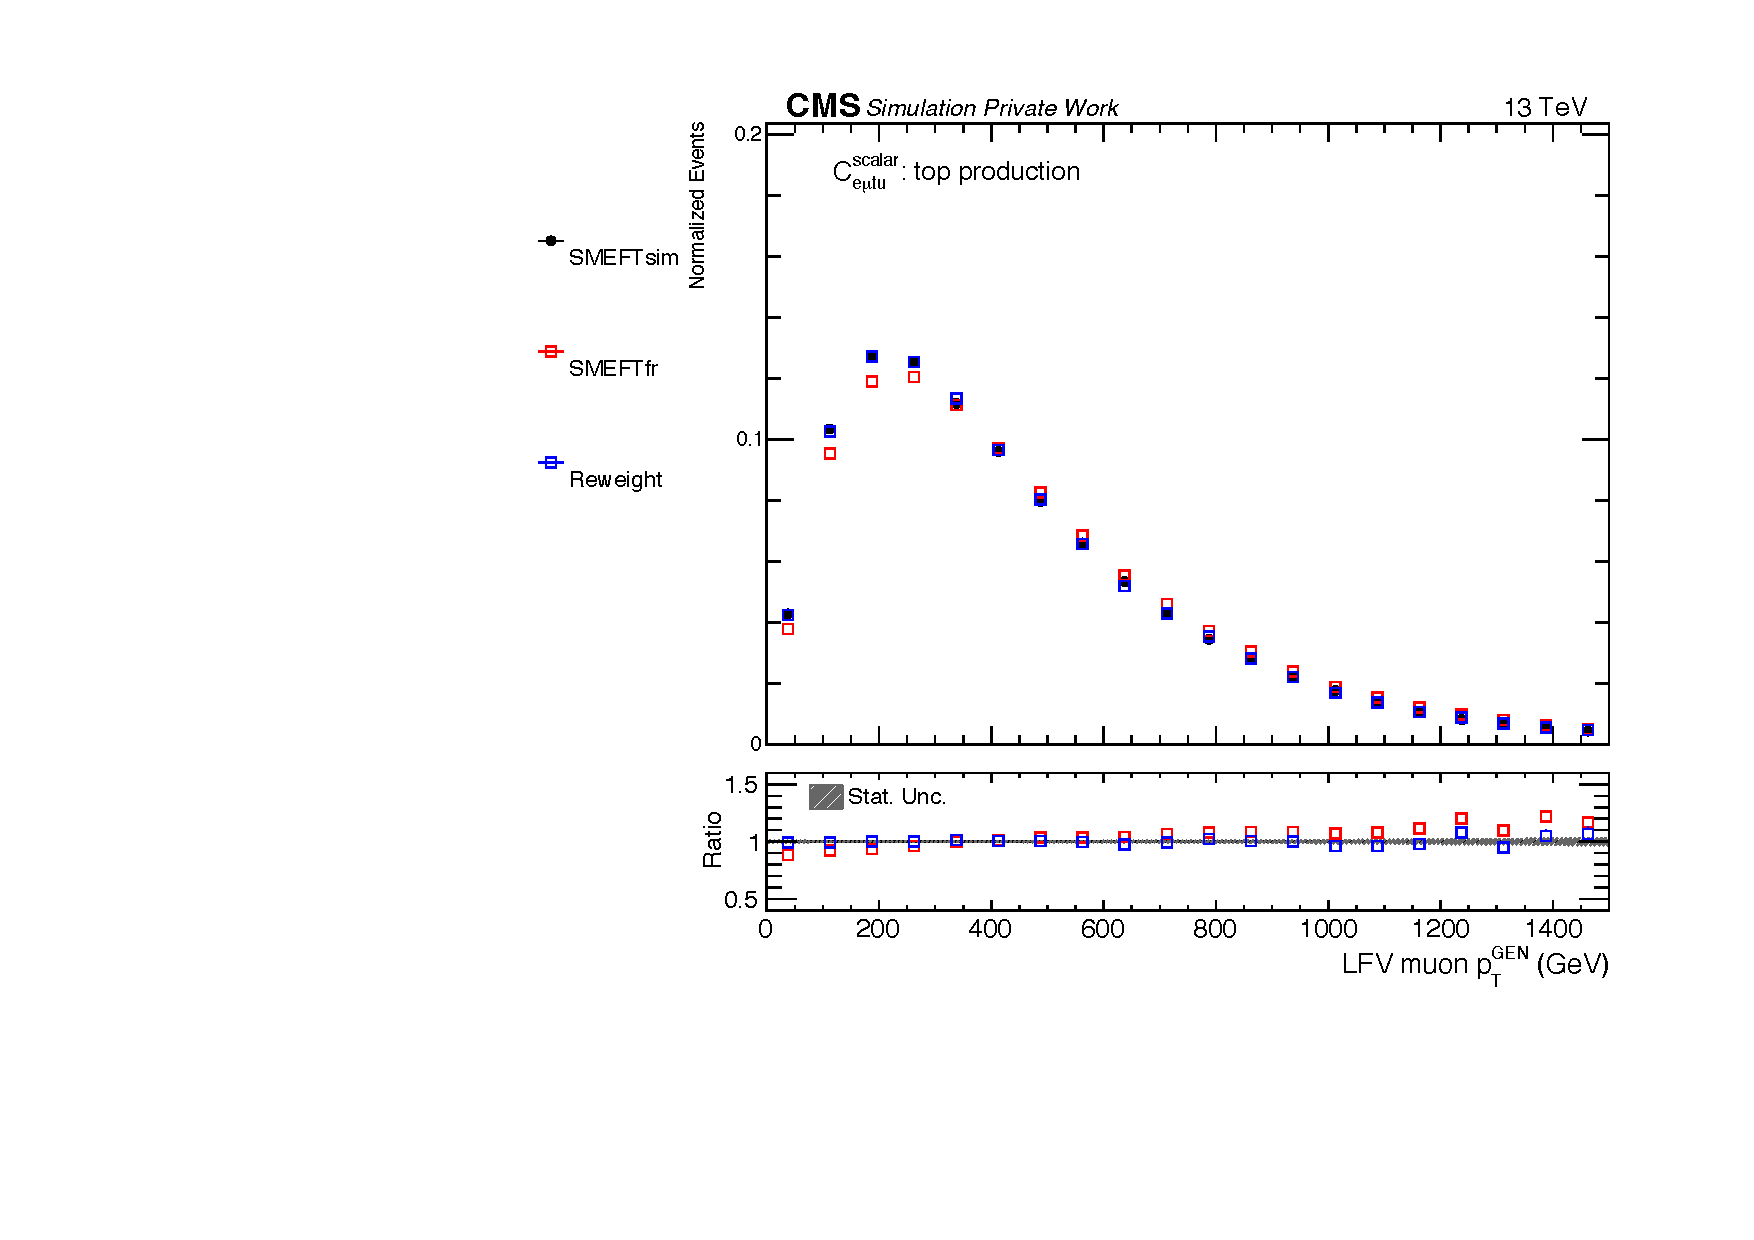
\includegraphics[width=0.48\textwidth]{figures/Part3/Samples/LFVmuPt}\\
 \end{tabular}
 \caption{Comparison of kinematic distributions at \ac{ME}-level produced by different models: LFV electron $\pt$ (left), LFV muon $\pt$ (right). The ``SmeftFR'' samples (shown in red curve) and ``SMEFTsim'' samples (shown in black curve) are statistically independent of each other. The ``Reweight'' (shown in blue curve) is produced by applying weights calculated by Equation~\ref{eq:2} to ``SmeftFR'' samples.}
 \label{fig:reweight}
 \end{center}
\end{figure}

In general, the calculations done by the \ac{ME} event generators are model-agnostic assuming the same \ac{EFT} configurations. In other words, models like SmeftFR or SMEFTsim~\cite{Brivio:2017btx} are expected to give the same or very similar results in terms of cross sections and four-momenta of final-state particles. Nevertheless, visible differences in kinematics have been observed and are shown in Figure~\ref{fig:reweight}. Furthermore, the cross sections predicted by SmeftFR v2 also yield more than 20\% difference relative to SMEFTsim due to a bug that was later fixed in SmeftFR v3. In light of these differences, the \ac{CMS} and \ac{ATLAS} Collaborations agreed to adopt the SMEFTsim model as the common standard. This decision was made after Ref.~\cite{CMS:2022ztx} has already been published, and Ref.~\cite{CMS:2022ztx} uses cross sections calculated by SmeftFR v2. To quantify the impact of the choice of models on kinematics, the following ratio is calculated for each event $i$,

\begin{equation}
\label{eq:2}
R_{\textsf{reweight}}^{i}=\frac{\omega_{\textsf{SMEFTsim}}^i}{\omega_{\textsf{SmeftFR}}^i},
\end{equation}

where $\omega^{i}_{X}$ is the per-event \ac{ME} weight calculated by \MG~using model $X$. Since SMEFTsim was not used by \ac{CMS} at the time when the signal samples were generated, $R_{\textsf{reweight}}$ are used to ``reweight'' the original samples generated using SmeftFR.

Due to the significant differences in kinematic distributions between top decay and production signals, \ac{MC} samples are generated separately for these processes. The cross sections for top production signals are taken directly from \MG~with SMEFTsim UFO as input. The event generation for top decay signals at the \ac{ME}-level takes two steps: (i) production of the SM $\ttbar$, and (ii) \ac{CLFV} decay of one of the top quarks. Therefore, the $\ttbar$ cross-section at \ac{NNLO} precision~\cite{Czakon:2011xx} is used to normalize the top decay signals,

\begin{equation}
\label{eq:3}
\sigma_{\textsf{CLFV}}^{\textsf{Top Decay}}=2\times\sigma_{\ttbar}^{\textsf{NNLO}}\times\mathcal{B}(\tto{q}),
\end{equation}

where q=\{u,c\}, and $\mathcal{B}(\tto{q})$ \cite{Kile:2008rp} can be expressed as,

\begin{equation}
\label{eq:4}
\mathcal{B}(\tto{q}) = 
 \begin{array}{l}
 \displaystyle
 \frac{|\WC{\textsf{vector}}{\emut{q}}|^2}{\Lam^4}\frac{\textsf{m}_\textsf{t}^5}{384\pi^3\Gam_{\textsf{t}}^{\textsf{SM}}} \\
 \displaystyle
 \frac{|\WC{\textsf{scalar}}{\emut{q}}|^2}{\Lam^4}\frac{\textsf{m}_\textsf{t}^5}{3072\pi^3\Gam_{\textsf{t}}^{\textsf{SM}}} \\
 \displaystyle
 \frac{|\WC{\textsf{tensor}}{\emut{q}}|^2}{\Lam^4}\frac{\textsf{m}_\textsf{t}^5}{64\pi^3\Gam_{\textsf{t}}^{\textsf{SM}}} 
\end{array}
\end{equation}

where $\textsf{m}_{\textsf{t}}$ and $\Gam_{\textsf{t}}^{\textsf{SM}}$ are taken to be 172.5 GeV and 1.33 GeV in this analysis, respectively. The choice of u or c quark in final states does not affect the cross sections of the top decay signals. The cross sections for all signal \ac{MC} samples are summarized in Table~\ref{tab:signal}. These cross-sections are used as a baseline to define the signal strength $\mu$, which is used to quantify the relative strength of the signals when their normalization change,

\begin{equation}
\mu(\textsf{C}/\Lam^2)=\frac{\sigma_{\textsf{CLFV}}(\textsf{C}/\Lam^2)}{\sigma_{\textsf{CLFV}}(\textsf{1}\TeV^{-2})}\propto(\textsf{C}/\Lam^2)^2.
\label{eq:signal_strength}
\end{equation}

\begin{table}[th]
\sffamily
\centering
\caption{Theoretical cross sections for top production and decay for each \ac{CLFV} coupling, calculated at $\WC{}{}/\Lam^2$ = 1 TeV$^{-2}$ by \MG~with SMEFTsim. Uncertainties related to \ac{PDF} and \ac{QCD} scale in \ac{ME} calculation are given ($\sigma^{+\text{scale}}_{-\text{scale}}\pm \text{PDF}$).}
\begin{tabular}{clll}
\toprule 
Lorentz Structure & Samples    & XS (fb) \\ \midrule
\multirow{3}{*}{vector} & top production via u quark & $460^{+81}_{-64}\pm6$ \\ 
  & top production via c quark & $33^{+5}_{-4}\pm6$ \\
  & top decay via u/c quark  & $32.0^{+0.8}_{-1.1}\pm1.3$ \\ \midrule
\multirow{3}{*}{scalar} &top production via u quark & $97^{+18}_{-14}\pm1$ \\ 
  & top production via c quark  & $6.3^{+0.9}_{-0.8}\pm1.4$ \\
  & top decay via u/c quark & $4.0^{+0.1}_{-0.1}\pm0.2$ \\ \midrule 
\multirow{3}{*}{tensor} & top production via u quark & $2140^{+370}_{-290}\pm30$ \\
  & top production via c quark & $164^{+22}_{-18}\pm27$ \\
  & top decay via u/c quark  & $187^{+5}_{-6}\pm8$ \\ \bottomrule
\end{tabular}
\vspace{-0.5em}
\label{tab:signal}
\end{table}

Steps other than the \ac{ME} calculation concerning signal \ac{MC} generation follow the \ac{CMS} standard, which is described in the following section.
%%%%%%%%%%%%%%%%%%%%%%%%%%%%%%%%%%%%%%%%%%%%%%%%%%%%%%%%%%%%%
%%%%%%%%%%%%%%%%%%%%%%%%%%%%%%%%%%%%%%%%%%%%%%%%%%%%%%%%%%%%%
\section{Background Samples}
\label{sec:Backgrounds}

The background processes are divided into two categories: (i) processes with three or more \emph{prompt} leptons in the final states are classified as ``\emph{prompt} background'', and (ii) other processes are classified as ``\emph{nonprompt} background''. The \emph{nonprompt} backgrounds in this analysis are modeled with a data-driven technique, which is discussed in \autoref{chap:Nonprompt}. The \ac{MC} samples listed in the ``\emph{nonprompt}'' category in Table \ref{tab:MCsample} are therefore only used for validations. 

Besides tZq, tHq, tHW, and tWZ processes, the \ac{NLO} \ac{PDF} set from NNPDF3.0~\cite{NNPDF:2014otw} is used in 2016 to generate background \ac{MC} samples. The \ac{NNLO} \ac{PDF} set from NNPDF3.1~\cite{NNPDF:2017mvq} is used for tZq while the \ac{LO} \ac{PDF} set from NNPDF3.0 is used for tHq, tHW, and tWZ in 2016. In 2017 and 2018, the \ac{NNLO} \ac{PDF} set from NNPDF3.1 was used to generate all the samples. 

The default choice of \ac{ME} event generator is \MG~v2.4.2 (v2.2.2 for 2016), which is used to generate all but ZZ, $\ttbar$H, and $\ttbar$ samples. These three samples are generated with \Pow~v2~\cite{Frixione:2007vw} instead. Samples with small contributions (tHq, tWZ, tHW, and low mass \ac{DY} ) are generated at \ac{LO} while other samples are generated at \ac{NLO}. Whenever possible and relevant, theoretical cross sections from high-order \ac{QCD} calculations are used. The references of these calculations are included in \ref{tab:MCsample}.

The \PY~v8.2~\cite{Sjostrand:2014zea} is used to model parton shower and hadronization. The CUETP8M1~\cite{CMS:2015wcf} was used in 2016 for underlying event tuning while the CP5~\cite{CMS:2019csb} was used in 2017 and 2018. The configurations of the \ac{MC} samples are summarized in Table \ref{tab:MCsample}. 

\begin{table}
\sffamily
\caption{Summary of the configurations of the \ac{MC} samples. DYM50 (DYM10to50) denotes a \ac{DY} sample with a dilepton invariant mass greater than 50 GeV (between 10 and 50 GeV). V includes W and Z bosons. The cross-sections for samples without a citation are taken directly from their event generators.}
\centering
 \resizebox{\linewidth}{!}{%
 \begin{tabular}{cccccc}
\toprule
Category & Process & Event Generator & Perturbative QCD& Tune & XS precision \\ \midrule
\multirow{7}{*}{\vtop{\hbox{\strut~~\emph{prompt}}\hbox{\strut background}}}  
 & WZ & \textsc{MadGraph} & NLO & CUETP8M1(CP5) & NLO~\cite{Campbell:2011bn} \\ 
 & ZZ & \textsc{powheg} & NLO & CUETP8M1(CP5) & NLO~\cite{Campbell:2011bn} \\
 &VVV & \textsc{MadGraph} & NLO & CUETP8M1(CP5) & NLO \\ 
 & $\ttbar$W, $\ttbar$Z & \textsc{MadGraph} & NLO & CUETP8M1(CP5) & NLO~\cite{Frederix:2021agh,Kulesza:2020nfh} \\
 & $\ttbar$H & \textsc{powheg} & NLO & CUETP8M1(CP5) & NLO~\cite{Kulesza:2020nfh} \\ 
 & tZq & \textsc{MadGraph} & NLO & CP5 & NLO \\
 & tHq, tHW, tWZ & \textsc{MadGraph} & LO & CUETP8M1(CP5) & LO \\
 \midrule
 \multirow{3}{*}{\vtop{\hbox{\strut \emph{nonprompt}}\hbox{\strut background}}}
 & $\ttbar$ & \textsc{powheg} & NLO & CUETP8M1(CP5) & NNLO~\cite{Czakon:2011xx} \\ 
 & DYM50 & \textsc{MadGraph} & NLO & CUETP8M1(CP5) & NNLO~\cite{Li:2012wna} \\
 & DYM10to50 & \textsc{MadGraph} & LO & CUETP8M1(CP5) & NLO~\cite{Li:2012wna} \\
 \bottomrule
 \end{tabular}}
 \label{tab:MCsample}
 \end{table} 
 
 All simulated events include a detailed simulation of the CMS detector response based on \textsc{Geant4}~\cite{GEANT4:2002zbu}, and are processed using the same \ac{CMS} event reconstruction software as used for the data.
 %%%%%%%%%%%%%%%%%%%%%%%%%%%%%%%%%%%%%%%%%%%%%%%%%%%%%%%%%%%%%
%%%%%%%%%%%%%%%%%%%%%%%%%%%%%%%%%%%%%%%%%%%%%%%%%%%%%%%%%%%%%
\section{Triggers}
\label{sec:Triggers}

The target final states of this analysis contain three prompt leptons, which make lepton triggers the most optical choice to select events. To achieve maximum acceptance, a combination of single-lepton, di-lepton, and tri-lepton triggers are used. These triggers are summarized in \autoref{chap:Triggers}. Events in simulated samples are required to fire at least one of the triggers listed in Table~\ref{tab:triggers16}-\ref{tab:triggers18}. Since multiple \acp{PD} are used to record data events and the orthogonality of these \acp{PD} is not guaranteed by the online selection criteria, the following trigger logic is implemented to remove the overlap between different \acp{PD}:

\begin{itemize}
\item Events in SingleMuon datasets are required to fire at least one of the triggers listed under ``SingleMuon''. 
\item Events in DoubleMuon datasets are required to fire at least one of the triggers listed under ``DoubleMu''. Events are removed if they also fire at least one of the triggers listed under ``SingleMuon''.
\item Events in ``MuonEG'' datasets are required to fire at least one of the triggers listed under ``MuonEG''. Events are removed if they also fire at least one of the triggers listed under ``SingleMuon'' or ``DoubleMu''.
\item Events in Single Electron datasets are required to fire at least one of the triggers listed under ``SingleElectron''. Events are removed if they also fire at least one of the triggers listed under ``SingleMuon'', ``DoubleMu'', or ``MuonEG''.
\item Events in DoubleEG datasets are required to fire at least one of the triggers listed under ``DoubleEG''. Events are removed if they also fire at least one of the triggers listed under ``SingleMuon'', ``DoubleMu'', ``MuonEG'', or ``SingleElectron''.
\item Events in EGamma datasets are required to fire at least one of the triggers listed under ``EGamma''. Events are removed if they also fire at least one of the triggers listed under ``SingleMuon'', ``DoubleMu'', or ``MuonEG''.
\end{itemize}